\subsubsection{Automated tests}
    Reply decided not to create automated tests but to rely on user tests instead.
    
    They stated that in the energy market scenario, users tests are more appropriate than automated tests for a variety of reasons.
    
    First of all, these data are very domain-specific, so writing a proper testing suite would require extensive domain knowledge.\\
    Secondly, most values come from external providers, so it is not possible to perform many actions if these values are detected as incorrect.\\
    Lastly, there is a notification system in place in case of critical errors (i.e. processes breaking and failing to complete).
    Reply has considered this notification system enough for this project.
    
    Further tests, such as the ones described in section \ref{section:tests:data}, have clearly shown that relying only on notifications and System Tests is not enough to assure the quality of the Data Warehouse.
    As a consequence, Reply has been requested to develop these tests during development, to shorten the delay between the deployment and the actual beginning of the data quality tests.
    
\subsubsection{Data correctness definition}
    An interesting aspect is the impossibility to determine if the data received are correct or not.
    
    Most data received are measurement taken by either operators or automated tools.
    In some other cases, data are the result of forecasting algorithms, developed by the provider themselves.
    
    Since there is no way to assert the correctness of the data received by the providers, the values shown on their websites are assumed to be correct.
    
    The only test that can be done is asserting that the information stored in the Data Warehouse, at the end of the download process, is identical to the information present on the websites.
    
\subsubsection{Priority vs non-priority data streams}
    All data streams have been categorized as priority or non-priority.
    
    Priority streams contain data needed by tools currently in use by the company.
    Having this data available is fundamental for running these tools on the cloud.
    
    On the other hand, some data has been marked as non-priority.
    These information are not currently used by any tool, but may be used in the future or for exploratory analysis.
    
    Given the low importance of having these data available in a short time, the only operation performed on them has been functional analysis, to identify if there are any issues with the data.
    A development date has, however, not been fixed: the ETL processes for these data stream will be developed during spare time or after all other priority data streams have been completed.
    
    The downside of this categorization is the lack of a precise time estimation for all the data streams.
    This is likely not to cause a consistent delay for a few data streams, but could become a problem for a high number of streams.
    
    Moreover, in several occasions Axpo employees had erroneously marked some data streams as non-priority, causing some confusion and forcing Reply to re-plan their work schedule.
    Changing these requirements naturally comports some delays, since we are requesting more work to be done before a deployment.
    
\subsubsection{Lack of formal documentation}
    A problem present in all development phases is the lack of a clear and formal documentation.
    Most of the information are in the heads of the developers, meaning that other people have either to ask them or to look directly at the code.
    The documentation present is represented in a non-clear way, usually using Excel sheets to annotate different types of information and comments.
    
    A more formal notation has been used, on the other hand, to represent the Data Warehouse structure.
    This notation, shown in Figures \ref{fig:reply:issues:dwh_diagram} and \ref{fig:reply:issues:dwh_diagram_table}, describes, however, only the columns present in each table, without specifying any relationship between them.
    Moreover, there is no clear distinction between fact tables (all the large boxes shown at the center of the Figure) and dimension tables (some of the small ones on the edges).
    
    \begin{figure}[p]
        \centering
        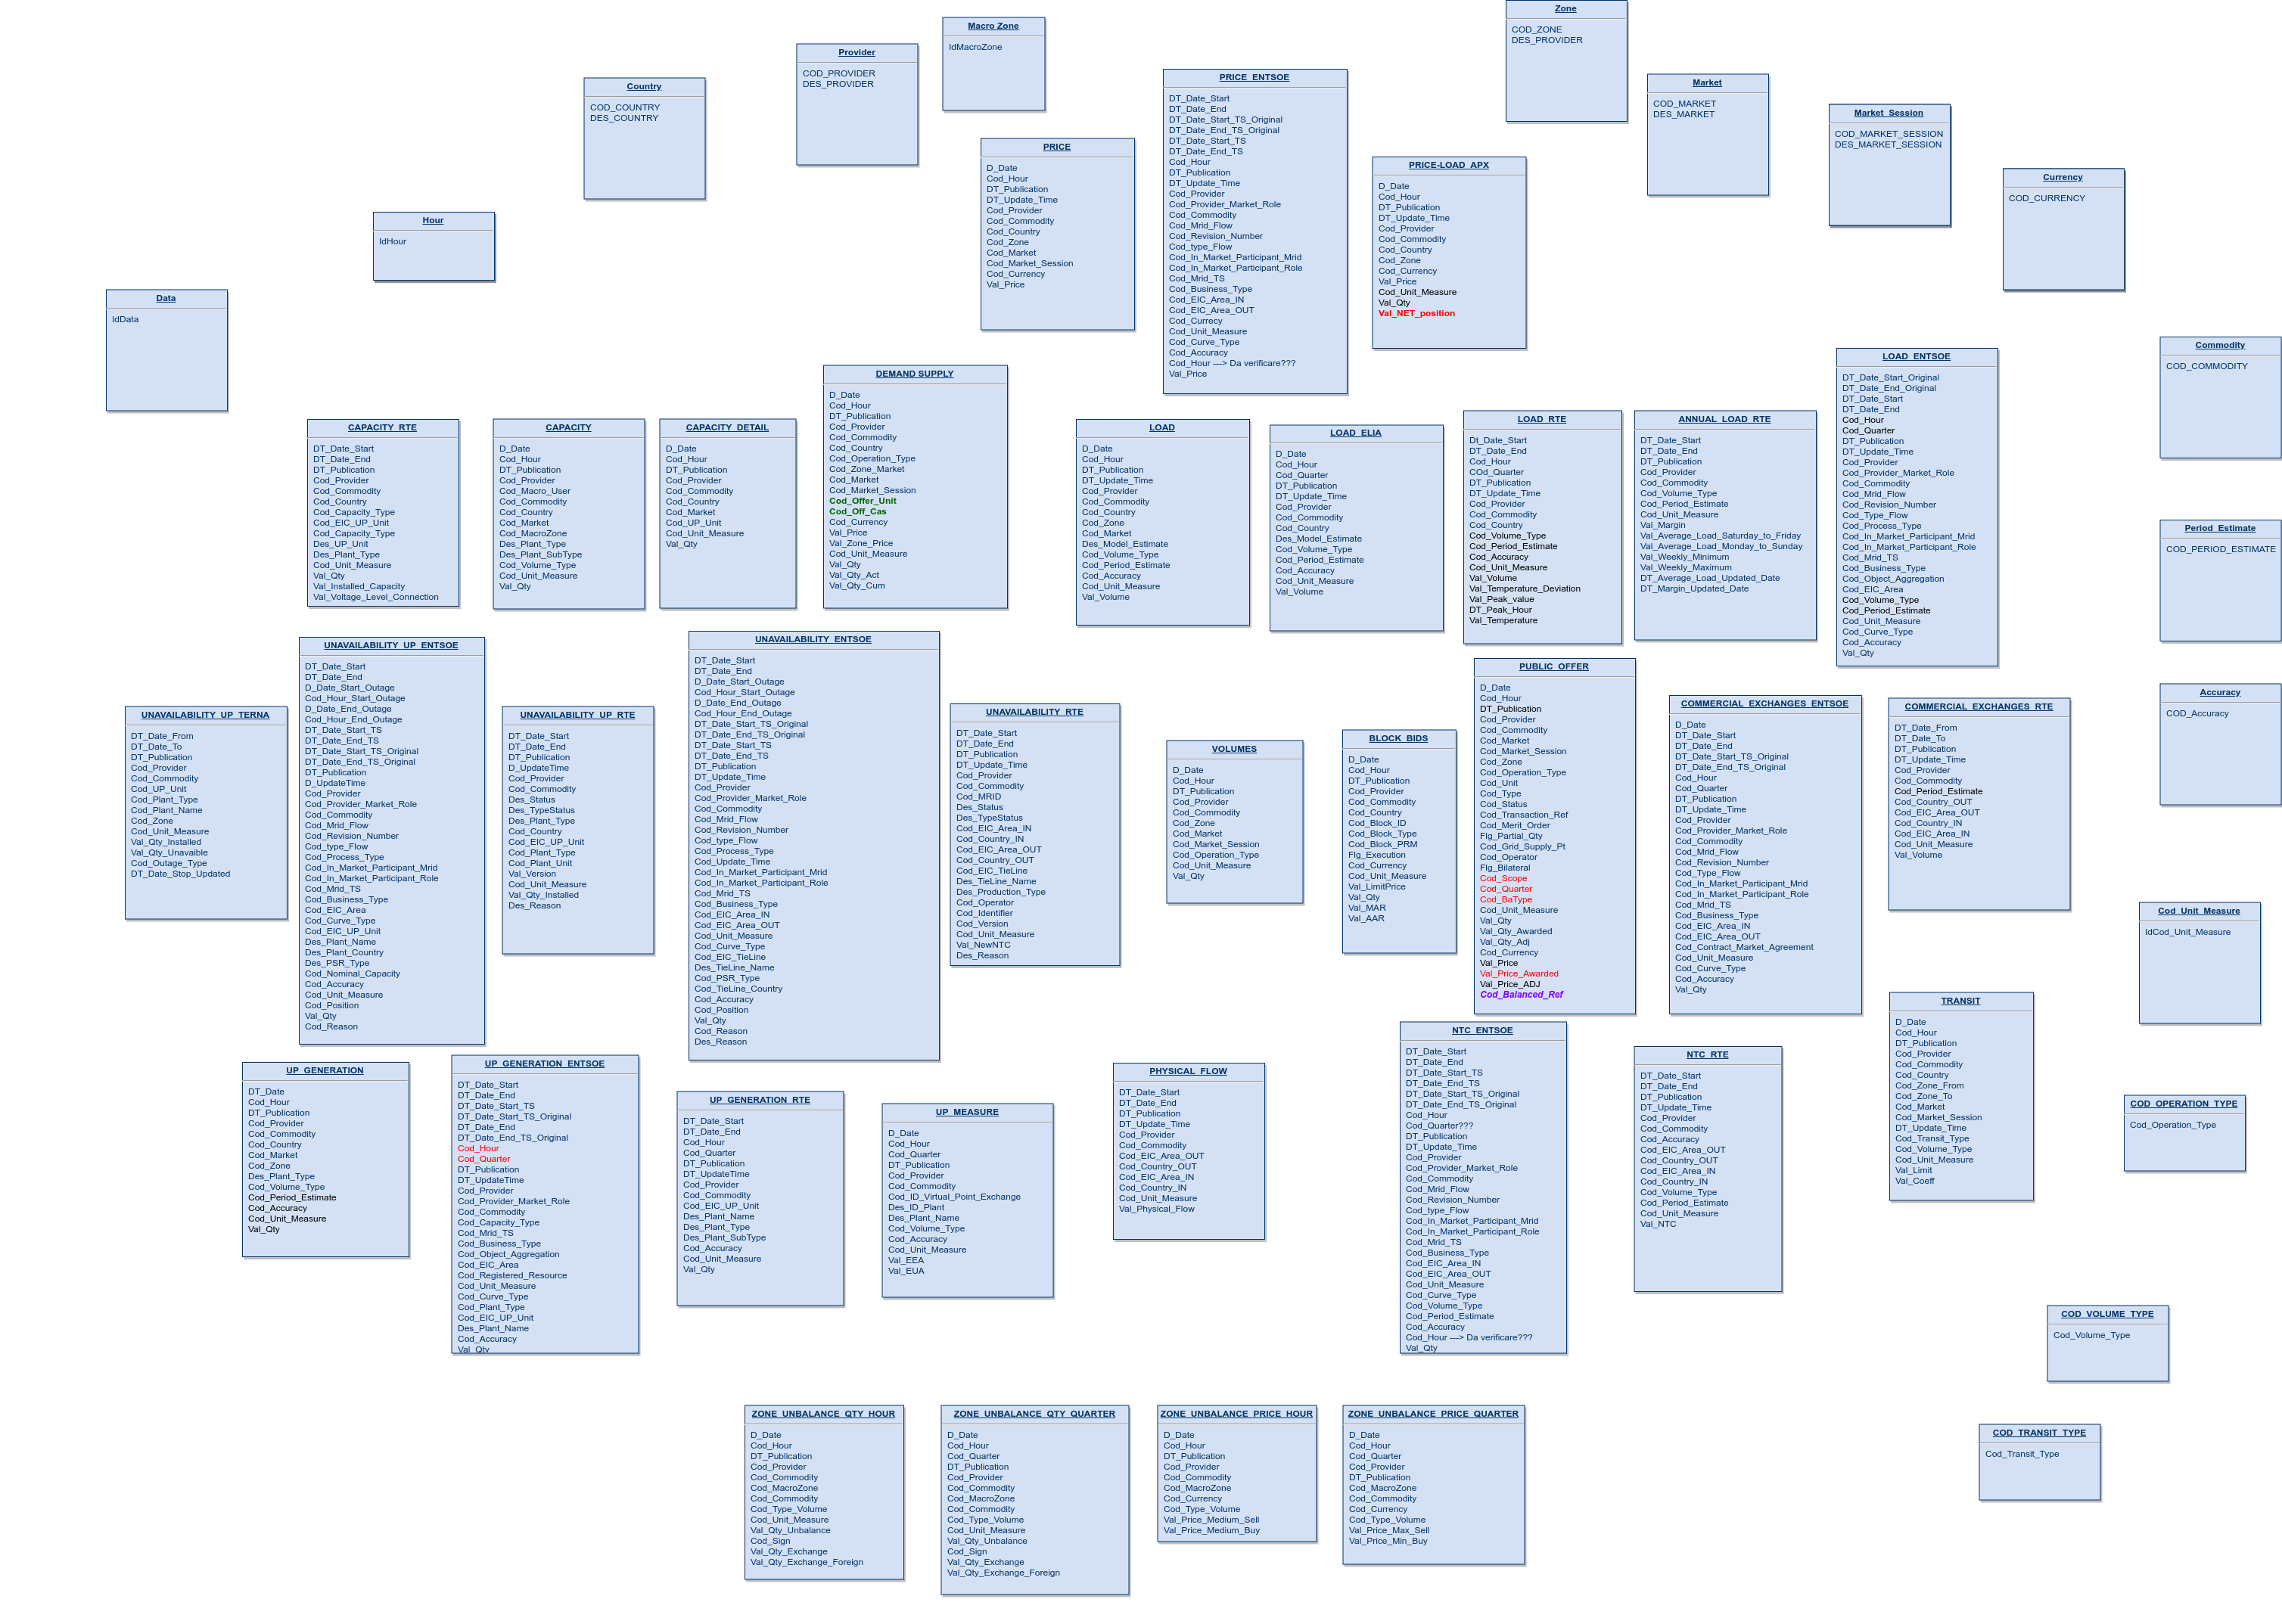
\includegraphics[width=\textwidth]{res/dwh_diagram.png}
        \caption{Diagram used for representing Data Warehouse structure.}
        \label{fig:reply:issues:dwh_diagram}
    \end{figure}
    
    \begin{figure}[p]
        \centering
        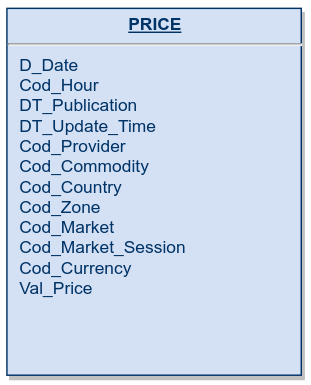
\includegraphics[width=.35\textwidth]{res/dwh_diagram_price.png}
        \caption{A single table from the Data Warehouse structure diagram.}
        \label{fig:reply:issues:dwh_diagram_table}
    \end{figure}
    
    An additional issue is that only the column names are reported, as shown in Figure \ref{fig:reply:issues:dwh_diagram_table}.
    Other relevant information, such as the data type for each column, are not shown.
    
    This design can, as a consequence, lead to confusion.